\chapter{Diseño y Desarrollo de la plataforma}
\label{chap:diseno_desarrollo}

En este capítulo se explicará todo el proceso de diseño y desarrollo de la plataforma, dando especial énfasis a la justificación de las decisiones tomadas y a la explicación de los distintos problemas que se han ido encontrando a lo largo del proceso. En concreto, se detallará el diseño de la base de datos, el desarrollo del \textit{backend} y el desarrollo del \textit{frontend}. No obstante, antes de entrar en detalle en cada una de estas secciones, se explicará el proceso inicial de desarrollo de la plataforma y se justificarán las tecnologías elegidas, cumplimentando así la sección \ref{sec:arquitectura_sistema} del capítulo \ref{chap:marco_teorico}.

% \textcolor{red}{Explicar que s'ha decidit fer un saas i una app web degut a les aventatges anteriorment esmentades.}

% \textcolor{red}{Ja s'ha dit que es farà servir React i Django i s'ha explicat breument com funcionen. Afegir el perquè d'aquestes eleccions.}

\section{Proceso inicial de desarrollo de la plataforma}
\label{sec:proceso_desarrollo}

El desarrollo de la aplicación web no surge de simplemente decidir qué tecnologías se van a utilizar y empezar a programar. Antes de comenzar a desarrollar la plataforma se ha llevado a cabo un proceso de diseño que ha permitido definir la arquitectura del sistema, las tecnologías a utilizar y el flujo de trabajo.

\subsection{Separación de tecnologías \textit{frontend} y \textit{backend}}

El primer paso que se ha realizado y una vez ya definido el objetivo de la aplicación y las funcionalidades que se querían implementar, se ha llevado a cabo un análisis de como estructurar la plataforma. Como ya se ha comentado en la sección \ref{sec:arquitectura_sistema}, se ha optado por una arquitectura dividida en dos partes: el \textit{backend}, incluyendo la base de datos, y el \textit{frontend}. No obstante, a pesar de que Django ofrece la posibilidad de crear ambas partes, se ha decidido utilizar React. Esta decisión ha supuesto un reto, ya que ha significado realizar un \textit{frontend} entero además de preparar una API en el \textit{backend} para que ambos se puedan comunicar. Sin embargo, esta decisión ha permitido crear una aplicación más escalable, flexible y, sobre todo, dinámica.

Django es un \textit{framework} que funciona del lado del servidor, lo que significa que cada vez que se quiere mostrar una página distinta, el servidor tiene que procesar la petición y devolver la página completa. De esta manera, cuando el usuario cambia de página, el servidor carga todos los recursos (HTML, CSS y JavaScript) y los rellena con los datos necesarios, sirviendo una página estática. Por el contrario, React es un \textit{framework} que funciona del lado del cliente, lo que significa que el servidor solo tiene que enviar los datos necesarios y el cliente se encarga de mostrar la información. Con esto, el servidor solo tiene que enviar los datos necesarios y el cliente se encarga de mostrar la información. Esto permite crear aplicaciones más dinámicas y rápidas, ya que no es necesario recargar la página cada vez que se quiere mostrar un nuevo contenido.

Este enfoque, a pesar de ser más complejo, es el estándar en la actualidad y es por este motivo que se ha optado por esta división de tecnologías.

\section{Diseño de la base de datos}
\label{sec:diseno_base_datos}

Para estructurar el proyecto, se ha optado por empezar definiendo la base de datos.

\begin{figure}
    \centering
    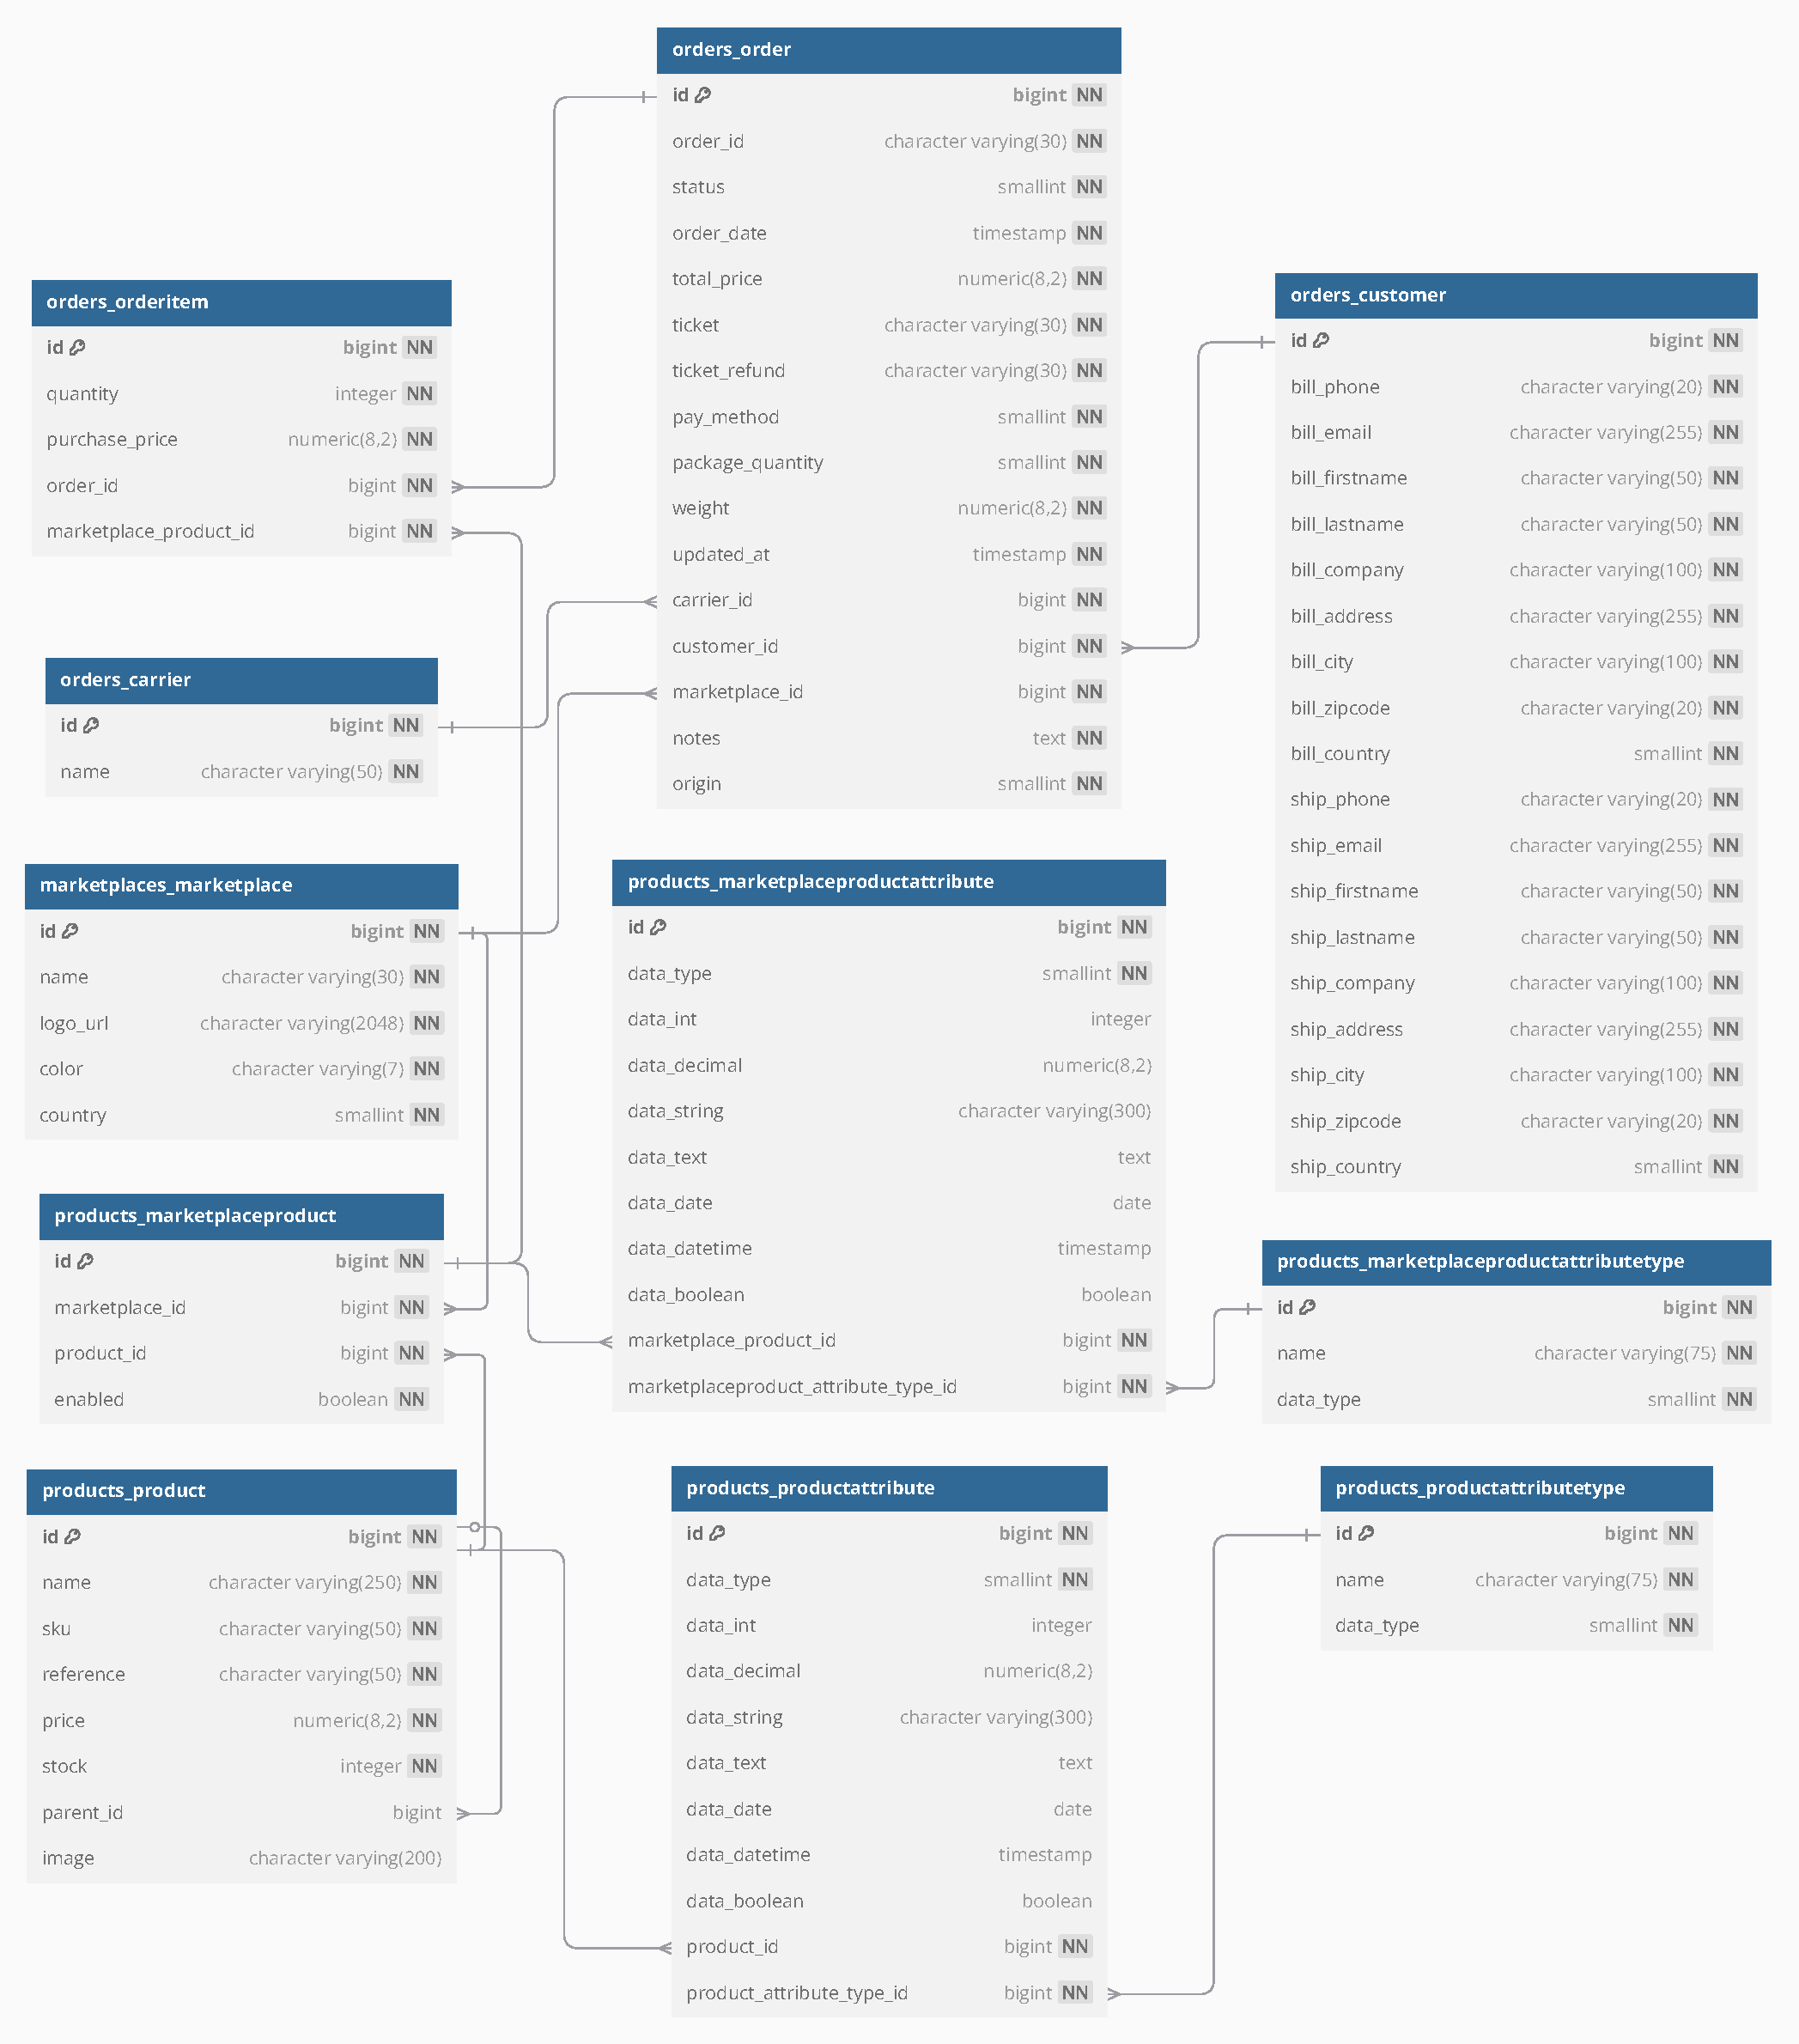
\includegraphics[width=0.98\textwidth]{figures/design_develop/database_diagram.pdf}
    \caption{Diagrama de la base de datos}
    \label{fig:diagrama_base_datos}
\end{figure}

\section{Desarrollo del \textit{backend}}


\section{Desarrollo del \textit{frontend}}